\documentclass[a4paper,12pt]{article}

\usepackage{graphicx}
\usepackage{float}
\usepackage{amsmath}

\usepackage[hyphens]{url}
\usepackage[margin=1in]{geometry}

\usepackage{subcaption}

\author{\vspace{1cm} \\
        Christopher Brown () \\
        Jack Croal (2062685) \\
        Cameron Houston (2082989) \\
        Alex Smith () \\
        Jok\=u bas Surgailis () \\
}

\date{}

\title{\vspace{4.0cm}Steering Wheel Display - Final Report}

\setlength\parindent{0pt}

\begin{document}

\maketitle

\thispagestyle{empty}

\begin{center}
\Large{Team Project EE4}
\end{center}

\begin{center}
\huge{Team Voltswagen}
\end{center}

\vspace{2.0cm}

\begin{center}

\includegraphics[width=8cm]{Figures/uni_logo.png}

\includegraphics[width=8cm]{Figures/ugr_logo_black.png}
\end{center}

\newpage
\clearpage
\pagenumbering{arabic}

\tableofcontents

% ====================================================================================================================

\newpage
\section{Introduction}
\label{sec:introduction}

As part of the Glasgow University Team Project EE4 course, a steering wheel display has been designed and prototyped for use within a University of Glasgow Racing car. This display allows the driver of the car to view live information from the CAN bus about the current status of the car. \\

Being the main client for the project, University of Glasgow Racing (UGR) have been involved throughout the design and manufacturing of the final product. UGR is the Glasgow University engineering team competing in Formula Student. Formula Student is a competition inspiring University students to design and build a single-seat race car. Each team’s race car is then put to the test against other teams from around the world. The Formula Student 2017 competition takes place on the 20th July 2017 at Silverstone Circuit, England. \\

It is important for the UGR race car driver to be able to view various information concerning the status of the race car because this allows the driver to understand how the car is performing. In order for the driver to be able to view this status information, a display is required. This display shows this status information such as the speed, RPM, gear number and coolant temperature by attaching directly to the car’s steering wheel. The values of these indicators were to be retrieved from the car's central CAN bus. \\

The following report covers the specifications of the completed steering wheel display, describing in detail each component and the reasons for the design. \\

\begin{figure}[H]
\begin{center}
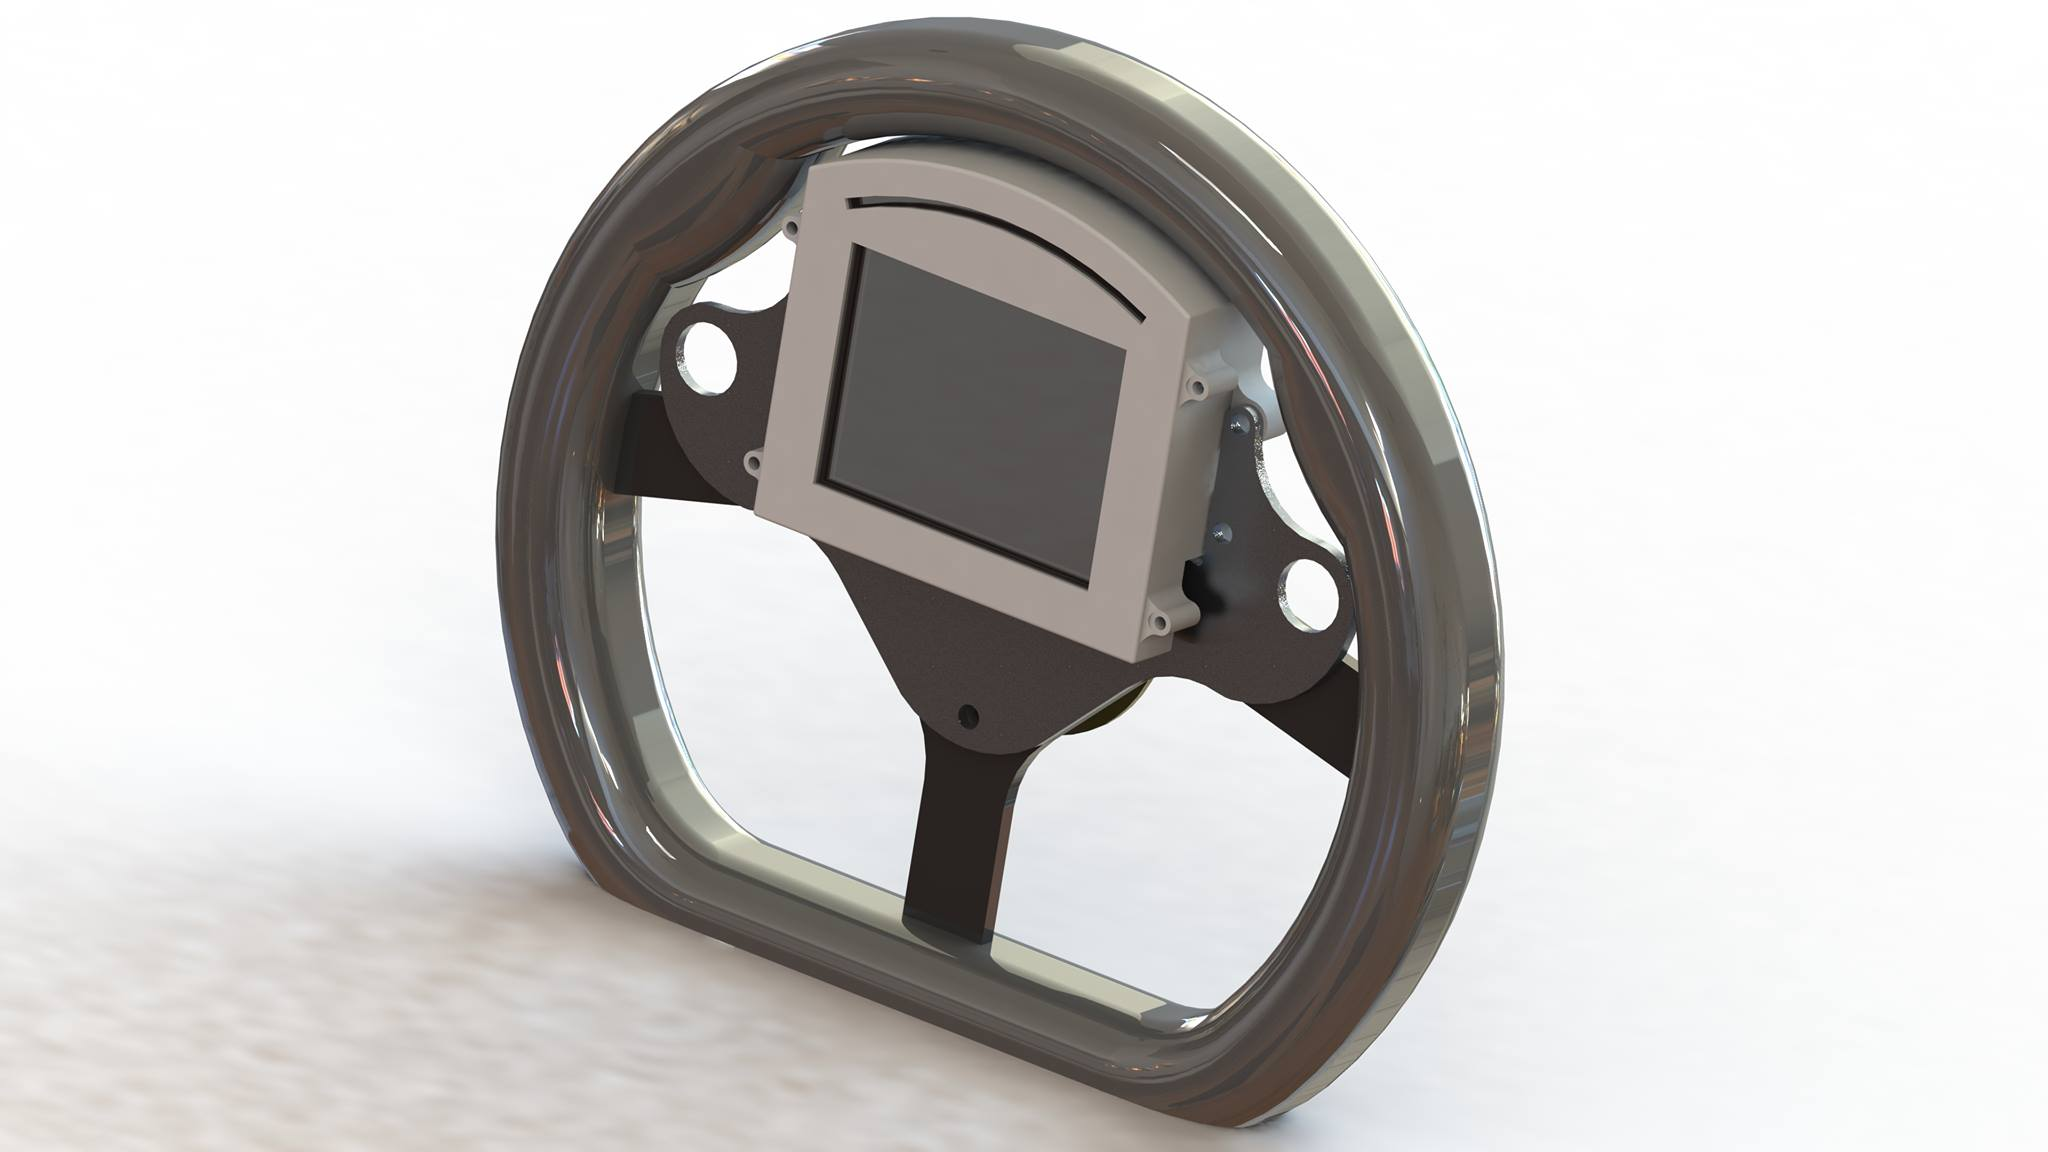
\includegraphics[width=12cm]{Figures/device_render_wheel.jpg}
\end{center}
\caption{SolidWorks render of outer enclosure attached to steering wheel}
\label{fig:device_render_wheel}
\end{figure}


% ====================================================================================================================

\newpage
\section{Device Requirements}
\label{sec:device_requirements}

This section covers the overall requirements for the device. These requirements were obtained from the UGR team. \\

The device connected to the main CAN bus of the car. This would

The steering wheel display was required to display the following status indicators to the driver:

\begin{enumerate}
  \item Speed (MPH).
  \item Gear number (including 'Neutral').
  \item Coolant temperature.
  \item Engine RPM.
  \item Battery Voltage.
  \item Warning symbols.
\end{enumerate}

In order to function properly, many aspects of the displayed values were required to be configurable by the user. This would increase the portability and flexibility of the device. These details are described further in Section \ref{sec:configuration_software}. \\

\textbf{Waterproofing} \\

It was required of the device to be IP67 compliant. This specifies that the device must be waterproof to 1m, and fully dustproof. This was because the steering wheel display needs to be operational in poor weather conditions. \\

\textbf{Mechanical Sturdiness} \\

The device was to be used in a mechanical environment, and therefore needed to be robust and resistant to high voltage spikes on the outside connections. \\

\textbf{Overheating} \\

The heat budget for the device was also important. The device was to be used for long periods of time, in possible warm temperatures. As a result, sufficient precautions for the dispersion of heat from the device needed to be taken.

% ====================================================================================================================

\newpage
\section{Device Overview}
\label{sec:device_overview}

The device consisted of four main components: the RPM LEDs, the microcontroller, the LCD screen and the CAN bus electronics. Figure \ref{fig:block_diagram} shows the overall block diagram of the device. \\

\begin{figure}[H]
\begin{center}
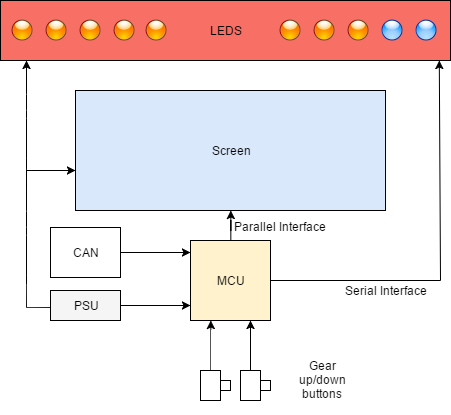
\includegraphics[width=12cm]{Figures/refined_block_diagram.png}
\end{center}
\caption{High level device block diagram.}
\label{fig:block_diagram}
\end{figure}


CAN bus is a serial communication technology used with motor vehicles to send information between individual systems and sensors. The car's central CAN bus was used to transmit the display information to the microcontroller and supply the device with power ($\sim$ 12 V DC). The CAN transceiver was used to convert the 5 V data lines of the CAN bus to the required 3.3 V input lines to the microcontroller. \\

The microcontroller would then process the data and output it the format required for the LCD display and RPM LEDs. \\

Two regulators were required in order to convert the 12 V DC voltage from the CAN bus to 5 V and 3.3 V power lines. The 5 V power line was used to power the RPM LEDs and the 3.3 V power line was used to power the microcontroller and LCD display. \\

% ====================================================================================================================

\newpage
\section{Electrical Design}
\label{sec:electrical_design}

When selecting components for the final device, each component was evaluated individually and in detail. In order to aid the construction process, each component needed to be in stock and readily available from a trusted distributor. The following section describes the requirements and final decisions for each component within the steering wheel display device. \\

\subsection{Microcontroller Requirements and Selection}
\label{sec:microcontroller}

The Microcontroller was to be chosen to minimise the number of peripheral elements required, whilst exhibiting sufficient processing power and I/O bus speed to provide to the LCD display, LEDs and other peripherals. As a result, the microcontroller was required to include:

\begin{enumerate}
  \item Sufficient number of digital output pins.
  \item CAN module.
  \item Fast digital I/O to update LCD display rapidly.
  \item Sufficient on-board memory.
\end{enumerate}

The microcontroller also had to be available in a package that could be soldered by hand. \\

Built-in writable EEPROM was also required on the microcontroller so that state could be stored when turning the device on and off. The EEPROM was to be used to store configuration details that were programmable by the user. The software for this feature is detailed in Section \ref{sec:CAN_software}. \\

The Atmel SAM3X8E ARM Cortex-M3 microcontroller was selected for the device. This microcontroller is used in the Arduino Due boards, and the Arduino Due was used as a basis for much of the design of the steering wheel display circuitry. The Quad Flat Package version was selected to allow for ease of soldering. \\

The Atmel SAM3X8E also included 2 CAN modules. This was useful because it allowed the testing of the CAN software without the use of more than one microcontroller; the microcontroller could send and receive to itself. \\

\subsection{LCD Display Requirements and Selection}
\label{sec:display}

The LCD display was to be used to display the majority of the car information to the driver, so it was very important for it to be able to display the appropriate information clearly and reliably. The requirements outlined by UGR are as follows:

\begin{enumerate}
  \item Clearly visible even in direct sunlight: brightness over 250 cd/$\textrm{m}^2$.
  \item Large enough to display all required information clearly.
  \item Easy to read at a glance.
  \item Available in a thin package, to reduce the depth of the overall device.
\end{enumerate}

As well as the operational requirements listed above, further requirements were included by the Voltswagen team in order to ensure the functionality of the device. This included a built-in display driver to make the software less complex and easier to write. This would allow the microcontroller to communicate with the display via the driver, instead of addressing individual registers on the display. Secondly, the team required clearly documented driver code to assist with programming. Lastly, as a result of the mechanical design of the outer enclosure, the display required metal or plastic tabs to allow it to fit properly within the device. \\

As a result of the requirements, the MIDAS MCT035AB0W320240LML TFT LCD display was selected \cite{display_datasheet}. This is a 320 x 240 pixel display, with an input voltage reuirement of 3.3 V. The display fitted all of the requirements given.

\subsection{LED Requirements and Selection}
\label{sec:LEDs}

In order to display the engine RPM of the car more clearly, coloured LEDs were a requirement of the client. These LEDs were to be above the screen and had to be easy to read even in direct sunlight. The client prefered to use different colours of LEDs depending on how high the engine RPM was. \\

It was decided to use Adafruit Dotstar LEDs for the RPM indicator \cite{dotstar_datasheet}. These devices use 2-wire SPI configuration which allow the user to configure the brightness and colour of individual LED’s in the strip. This is accomplished by using an embedded microcontroller inside the LED. 12 LEDs were implemented in the steering wheel display device. Figure \ref{} shows the final Dotstar LEDs at full engine RPM. \\

After reviewing steering wheel display implementations from previous official Formula One racing cars, it was decided to use a three colour scheme of Green, Red, and Blue, in order of increasing RPM \cite{bsim_racing, daily_mail_1}. This ensured the device complied with the current trends in high-end steering wheel display design.

\subsection{Power Requirements and Selection}
\label{sec:PSU}

Once the main components were selected, the overall power consumption of the device could be evaluated. Table 1 shows the quoted power requirements of the main components within the device.

\begin{center}
\begin{tabular}{ | c | c | c | c | c | c | }
\hline
 Component & Voltage (V) & Current (A) & Quantity & Power Consumption (W) \\
\hline
 LCD Display & 3.3 & 0.525 & 1 & \\
\hline
 Microcontroller & 3.3 & 0.8 & 1 & \\
\hline
 LEDs & 5 & 0.02 & 12 & \\
\hline
\end{tabular}
\par
\bigskip
Table 1: Power Consumption of Device.
\end{center}

The components were to be housed in a closed container, therefore, the generated heat needed to be assessed to ensure that the final product will not overheat in its environment. The calculations for the heat from various components have been included in Appendix \ref{}. \\

After completion, the power requirements of the device were tested in a laboratory setting. It was found that the device only sourced 0.2 A at 12 V supply voltage. This was a lower value than calculated during the design phase. This result may make the device more resilient to overheating.

\subsection{Other Components}
\label{sec:other_components}

All components on the device were surface mount.

% ====================================================================================================================

\newpage
\section{Software Design}
\label{sec:software_design}

As well as the device electronics, the quality of the software is also of high importance in order to ensure the device runs smoothly and meets all requirements. As a result, the software needed to be highly maintainable and comprehensive.

\subsection{CAN Software}
\label{sec:CAN_software}

CAN (Controller Area Network) was used throughout the UGR racing car in order to pass information between the different components. The steering wheel display was designed to read the relevant car status information from the CAN bus and output this data on its display at real-time speeds. \\

The CAN software was implemented using the Due CAN library \cite{due_can}. This is a CAN bus library that is compatible with the Arduino Due board. A large amount of information was sent over the car’s CAN bus, however not all of this information was relevant to the device. The role of the CAN software was to filter out the irrelevant information, only sending useful information to the device peripherals. The library allowed various CAN mailboxes to be set up, each with a different CAN identifier, that would call the appropriate function to handle the data in the CAN frame. The LCD screen and RPM LEDs could then be updated with the filtered car information via the display software described in Section \ref{sec:display_software}. \\

The CAN bus requires a set of CAN frame identifiers in order to sort the bus information. Although these CAN identifiers were already specified by UGR, they were subject to change in the future. As a result, these identifiers had to be designed to be configurable on the device. Configurable CAN identifiers were implemented in the diagnostics software using the configuration menu described in Section \ref{sec:configuration_software}.

\subsection{Display Software}
\label{sec:display_software}

The display software was used to output the relevant car information to the device peripherals: LCD display and RPM LEDs. The main requirement of this part of the software was that it had to be clear and easy to view. As a result, the colour scheme chosen was black and white, and custom fonts were used to improve the visibility of the displayed values. \\

This software involved the development of a custom driver for the LCD display. This driver was designed to allow text and symbols to be output in a specified location on the LCD display, allowing for ease of configurability of the display output. Basic functions allowing text and images to be display anywhere on the screen at specified font sizes were implemented. The main display software would then make use of the driver to output values onto the LCD display. Figure \ref{fig:display} shows the display software outputting example car information. \\

\begin{figure}[H]
\begin{center}
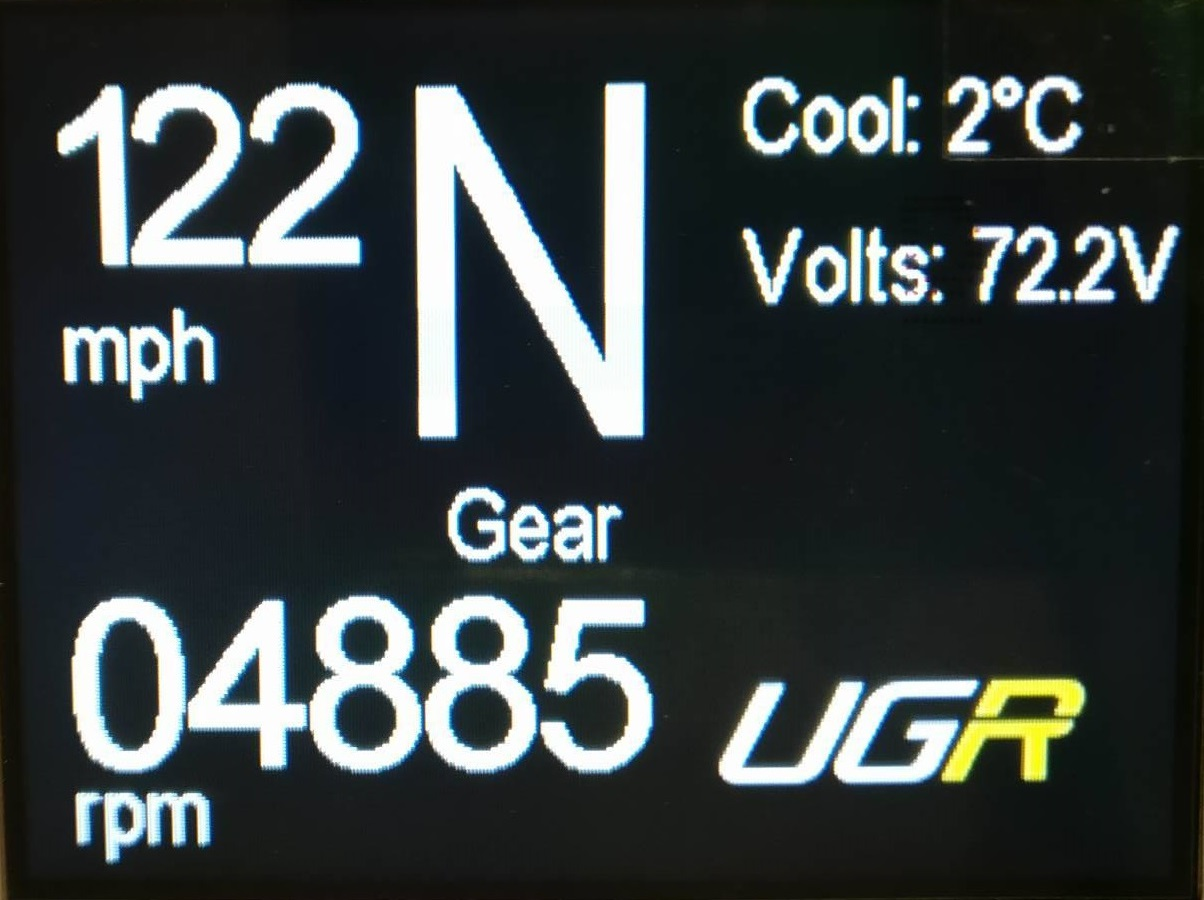
\includegraphics[width=10cm]{Figures/display.jpg}
\end{center}
\caption{Device shown in Display Mode}
\label{fig:display}
\end{figure}


DotStar LEDs were used to display the RPM of the engine, as mentioned in Section \ref{sec:LEDs}. This was implemented in software using the Adafruit DotStar Arduino Library, which allowed the colour and brightness of the LEDs to be easily configured.

\subsection{Diagnostics Software}
\label{sec:diagnostics_software}

In order to aid with the debugging of the device with respect to the CAN frames, a Diagnostics Mode was implemented. This could be activated by pressing both gear buttons on startup of the device for 3 seconds. When activated, a verbose representation of the CAN bus would be printed onto the LCD display. Figure \ref{} shows an example of the CAN diagnostics software in operation. Although this was useful for the writing of the CAN software, it was also designed to be used by a mechanic for debugging the overall car’s CAN bus by allowing the screen to act as a CAN frame probe. \\

Up to 30 different CAN frames were able to be displayed in diagnostics mode. Only 6 CAN frames were to be displayed on the screen at one time, therefore, 6 pages of CAN frames were implemented. The next and previous pages could be viewed by pressing the right and left gear buttons respectively.

\subsection{Configuration Software}
\label{sec:configuration_software}

Some aspects of the device were required by the client to be configurable, as previously discussed. Specifically:

\begin{enumerate}
  \item Speed units (MPH or KPH).
  \item Threshold for coolant temperature error symbol to show.
  \item CAN frame identifiers for use in the diagnostics software.
\end{enumerate}

A configuration menu through Serial USB when the device is plugged into a computer was therefore implemented. This serial interface allowed the user to configure the various details of the device through a command prompt interface. Figure \ref{} shows an example of the configuration software being used.

%\begin{figure}[H]
\begin{center}
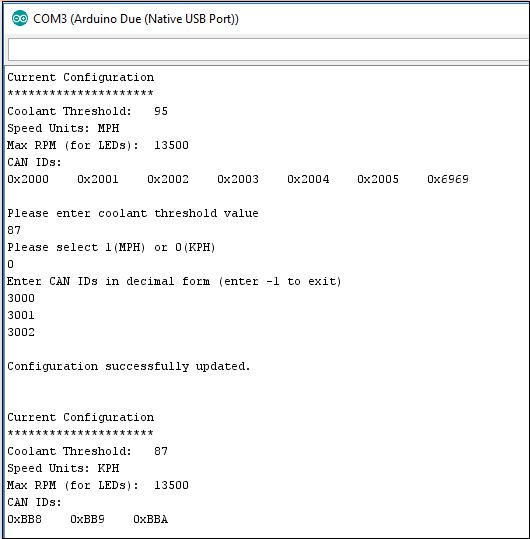
\includegraphics[width=12cm]{Figures/configuration_software.png}
\end{center}
\caption{Example of Configuration Mode in use.}
\label{fig:configuration_software}
\end{figure}


State was stored on the device using the microcontroller's built-in EEPROM. This was implemented in software using the Due Flash Storage library \cite{due_flash_storage}. When activated, by plugging the device into a computer with the serial input/output enabled, the user would be able to select personalised configuration options. After configuration the new values would automatically be loaded into the software when the device is next turned on. If the device has not yet been configured, then default values are loaded into the software instead.

% ====================================================================================================================

\newpage
\section{Mechanical Design}
\label{sec:mechanical_design}

As well as the electrical components, the device required mechanical design in order to meet the requirements of the customer.

\subsection{Outer Enclosure}
\label{sec:outer_enclosure}

In order to house the device components, an outer enclosure needed to be constructed. The requirements from the UGR team are as follows:

\begin{enumerate}
  \item Must mount onto the current UGR wheel.
  \item Must be lightweight.
  \item IP67 Watertight.
  \item Must allow for correct use of the wheel, and therefore be constrained dimensionally.
  \item Must incorporate shifting buttons as they are in the same area of the wheel.
\end{enumerate}

The outer enclosure was developed using SolidWorks. An expanded render of the outer enclosure is shown in Figure \ref{fig:device_render_expanded}. This was 3D printed using through the University.

\begin{figure}[H]
\begin{center}
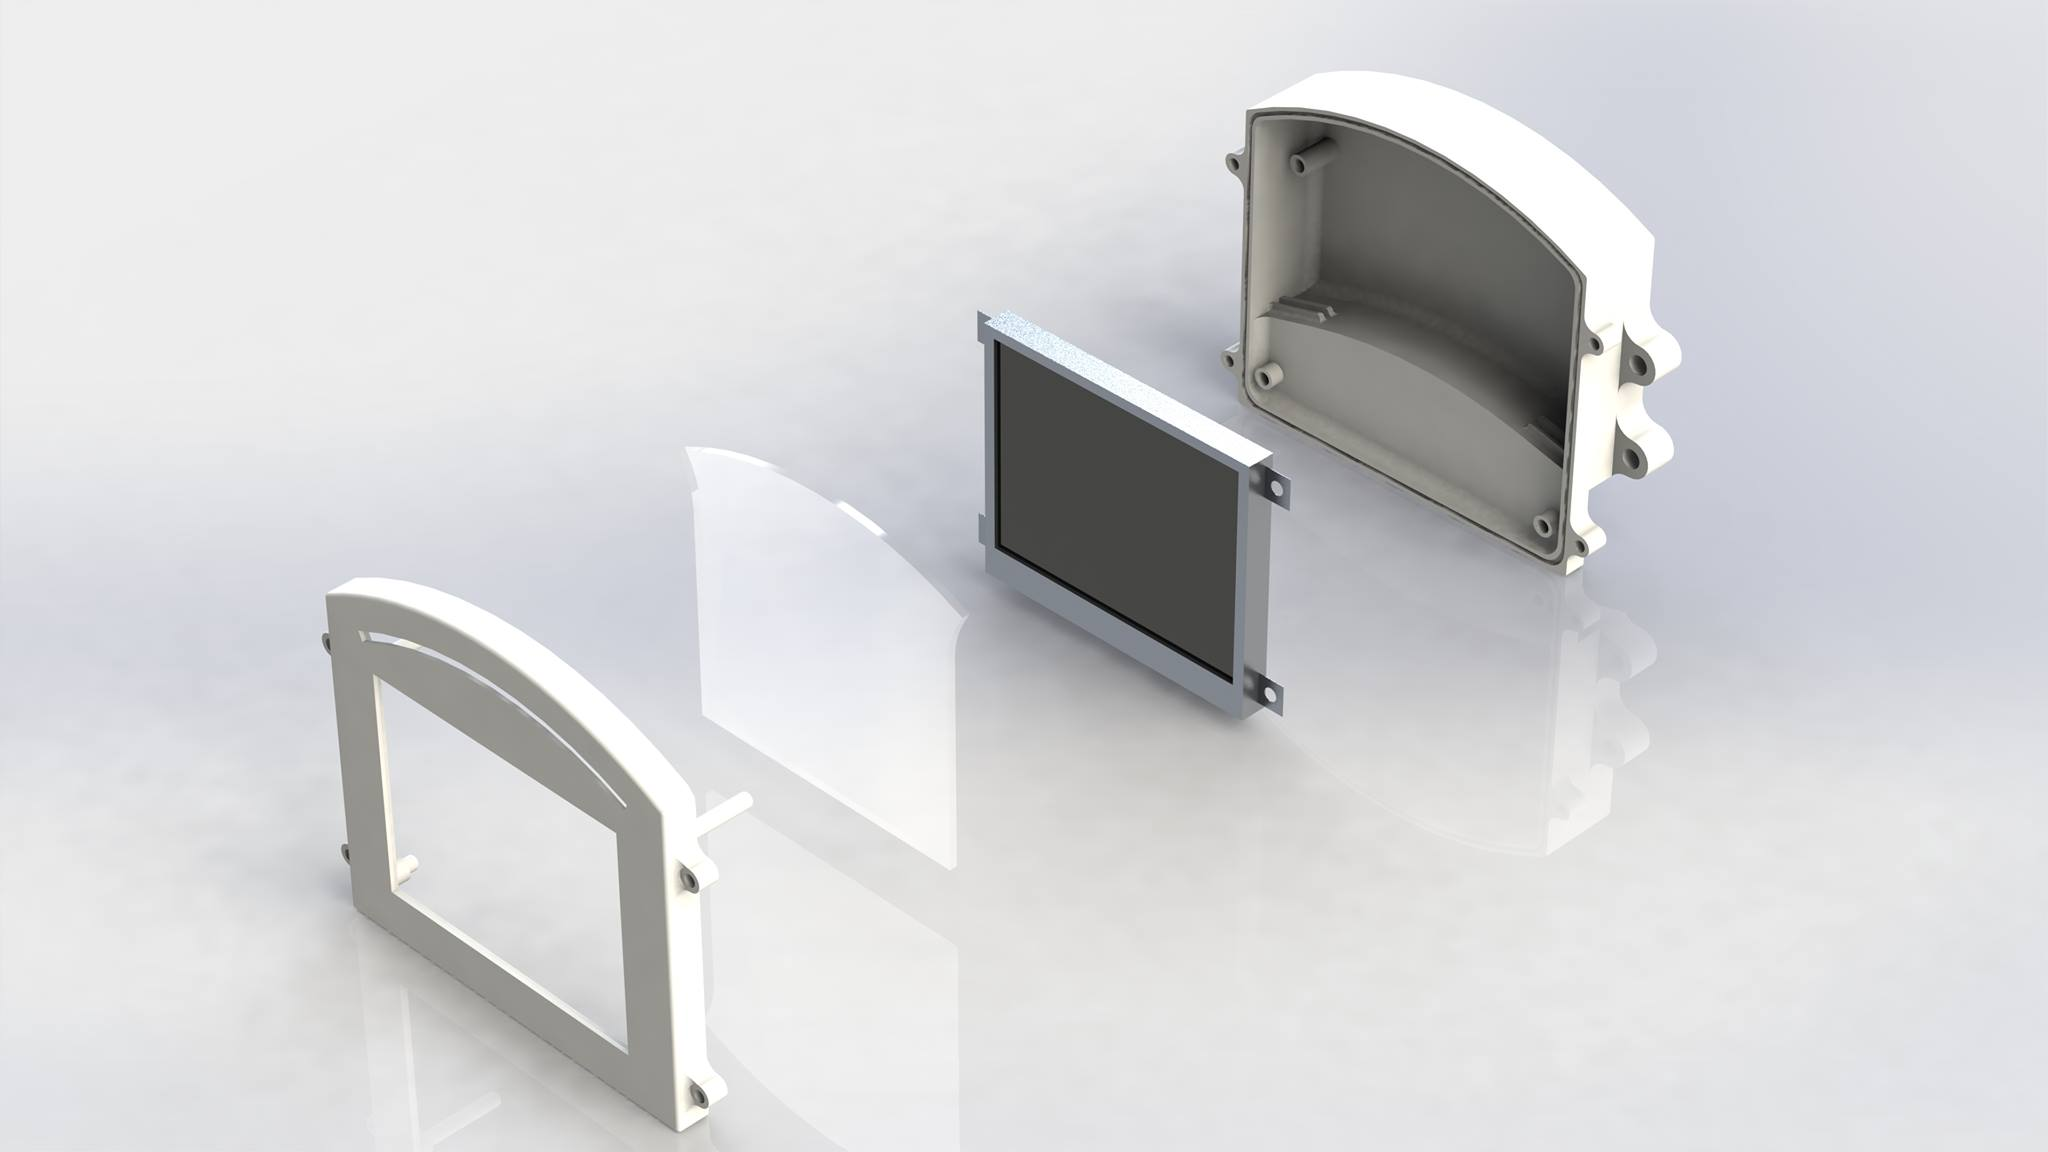
\includegraphics[width=12cm]{Figures/device_render_expanded.jpg}
\end{center}
\caption{SolidWorks render of outer enclosure and display.}
\label{fig:device_render_expanded}
\end{figure}


\subsection{Printed Circuit Board}
\label{sec:printed_circuit_board}

As a result of the space constraints, the PCB needed to be able to fit within the design of the outer enclosure. This required the PCB to be of a specific shape, with the use of small electrical components consistently. The shape of the PCB within the context of the outer enclosure is described in Figure \ref{fig:PCB}.

\begin{figure}[H]
\centering
\begin{subfigure}{.5\textwidth}
  \centering
  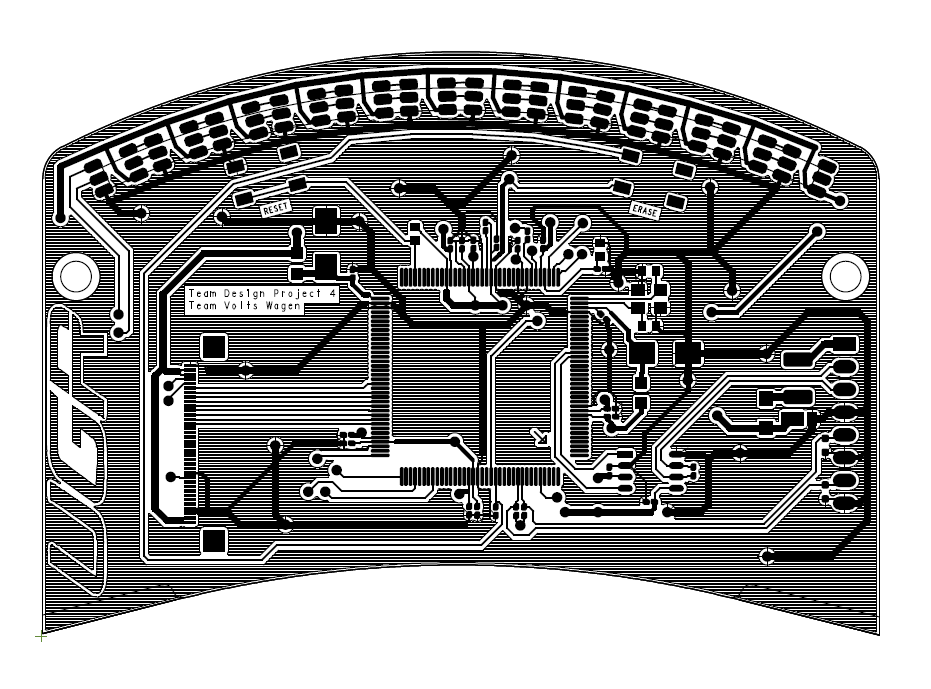
\includegraphics[width=8.5cm]{Figures/PCB_front.png}
  \caption{PCB design front view.}
  \label{fig:PCB_front}
\end{subfigure}%
\begin{subfigure}{.5\textwidth}
  \centering
  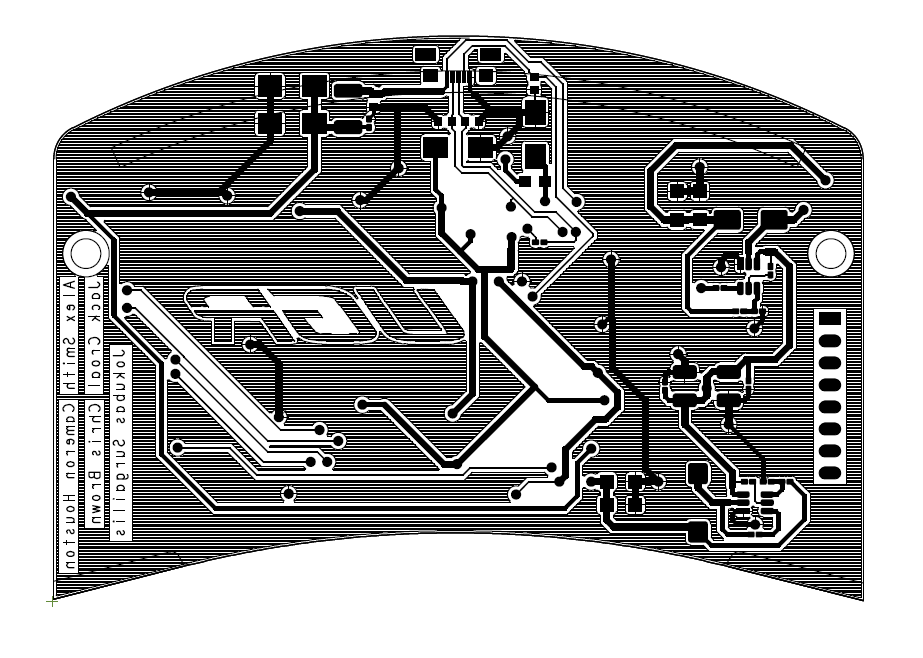
\includegraphics[width=8.5cm]{Figures/PCB_back.png}
  \caption{PCB design rear view.}
  \label{fig:PCB_back}
\end{subfigure}
\caption{Overall PCB design for case.}
\label{fig:PCB}
\end{figure}

% ====================================================================================================================

\newpage
\section{Costs and Expenditure}
\label{sec:cost}

\subsection{Cost for fabrication of the device}
\label{sec:device_cost}

\subsection{Total cost for development}
\label{sec:total_cost}

% ====================================================================================================================

\newpage
\section{Future Improvements}
\label{sec:future_improvements}

This section describes any possible improvements that could be made to the final device. These features were not included in the design due to various time and resource constraints. Although the final device met the functional and nonfunctional requirements presented by the UGR team, we believe these future improvements could further improve the capabilities of the overall device.

\subsection{Professionally Fabricated Board}
\label{sec:future_improvement_1}

The Printed Circuit Board was manufactured in Glasgow University and could have been reduced in size, had it been manufactured externally. This was considered during the project design, however it was decided to not get the PCB professionally made due to the extra cost and complication of the device fabrication. A quote of £100 from ‘PCB Train’ was obtained \cite{pcb_train}. Making use of the facilities within the University reduced the project risk because it allowed PCBs to be re-designed and fabricated within a short timeframe (1-4 days, compared to the 2-week quote for a professionally made PCB).

\subsection{More Robust Power Supply Unit}
\label{sec:future_improvement_2}

\subsection{Faster Parallel Output}
\label{sec:future_improvement_3}

% ====================================================================================================================

\newpage
\section{Project Management}
\label{sec:project_management}

% ====================================================================================================================

\newpage
\bibliographystyle{ieeetr}
\bibliography{bibliography}

\end{document}

































